\documentclass{beamer}
\usepackage[utf8]{inputenc}
\usepackage[T1]{fontenc}
\usepackage{graphicx}
\usepackage{multicol}
\graphicspath{{./images/}}

\usetheme{Arguelles}

\title{Using FPGAs to Perform Cryptanalytic Attacks on Random Number Generators}
\subtitle{}
\date{27/5/2021}
\author{Andreas Stocker}
\institute{University of Nicosia\par\email{andreas@stockers.org}}

\begin{document}

  \frame[plain]{\titlepage}
  

  \begin{frame}
    \frametitle{Abstract}
    \framesubtitle{The purpose of this paper}

    This paper combines two somewhat unrelated subjects, FPGAs and cryptanalysis.
    It provides background on both of these subjects and then culminates
    in an experiment that combines the two.
  \end{frame}

  \Section{FPGAs}

  \begin{frame}
    \frametitle{What are FPGAs?}


    \begin{multicols}{2}

    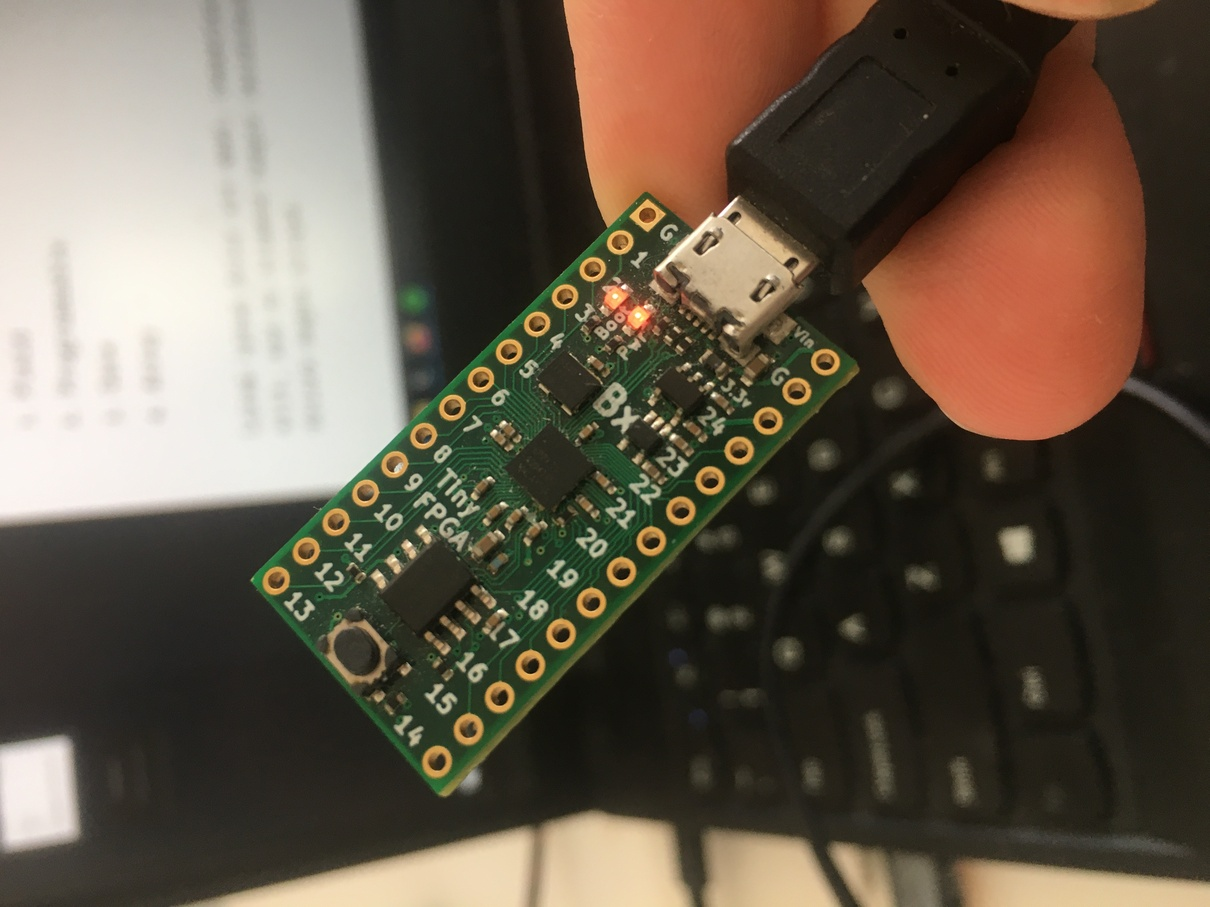
\includegraphics[scale=0.15,angle=-90]{tinyfpga-bx}
    
    \vfill
    
    \vspace*{\fill}
    
    \AlegreyaExtraBold FPGA \ttfamily stands for:
    \begin{enumerate}
      \item Field
      \item Programmable
      \item Gate
      \item Array
    \end{enumerate}
    
    \vspace*{\fill}

    \end{multicols}
    
  \end{frame}
   
  \ThankYou
  \begin{frame}[plain,standout]
    In combination with \textit{plain},\par
    it makes a nice thank-you slide!

    \vfill{Generated using \textit{Beamer} and the \textit{Arguelles} Theme}
  \end{frame}

\end{document}
